\documentclass[zavrsnirad]{fer}
% Dodaj opciju upload za generiranje konačne verzije koja se učitava na FERWeb
% Add the option upload to generate the final version which is uploaded to FERWeb


\usepackage{blindtext}
\usepackage{tikz}
\usetikzlibrary{arrows.meta, shapes.geometric, positioning}

%--- PODACI O RADU / THESIS INFORMATION ----------------------------------------

% Naslov na engleskom jeziku / Title in English
\title{Mobility management of a Raspberry Pi device in a mobile network}

% Naslov na hrvatskom jeziku / Title in Croatian
\naslov{Upravljanje pokretljivosti Raspberry Pi uređaja u mobilnoj mreži}

% Broj rada / Thesis number
\brojrada{1344}

% Autor / Author
\author{Matija Alojz Stuhne}

% Mentor 
\mentor{izv. prof. dr. sc.\@ Marin Vuković}

% Datum rada na engleskom jeziku / Date in English
\date{June, 2024}

% Datum rada na hrvatskom jeziku / Date in Croatian
\datum{lipanj, 2024.}

%-------------------------------------------------------------------------------


\begin{document}


% Naslovnica se automatski generira / Titlepage is automatically generated
\maketitle


%--- ZADATAK / THESIS ASSIGNMENT -----------------------------------------------

% Zadatak se ubacuje iz vanjske datoteke / Thesis assignment is included from external file
% Upiši ime PDF datoteke preuzete s FERWeb-a / Enter the filename of the PDF downloaded from FERWeb
\zadatak{hr_0036540079_73.pdf}


%--- ZAHVALE / ACKNOWLEDGMENT --------------------------------------------------

\begin{zahvale}
  % Ovdje upišite zahvale / Write in the acknowledgment
\end{zahvale}


% Odovud započinje numeriranje stranica / Page numbering starts from here
\mainmatter


% Sadržaj se automatski generira / Table of contents is automatically generated
\tableofcontents


%--- UVOD / INTRODUCTION -------------------------------------------------------
\chapter{Uvod}
\label{pog:uvod}

\section{Motivacija}

S Obzirom na jednostavnu prenosivost te široki spektar primjena, računalo Raspberry Pi izuzetno je
popularan dio IoT svijeta. Kao takav, zbog prisutnosti brojnih dodataka i proširenja, moguće ga je koristiti
i u mobilnoj mreži. U kombinaciji s proširenjem koje služi kao modem, Raspberry Pi uređaj postaje
korisnička oprema u mobilnoj mreži. No, postavlja se pitanje koliko je ovaj način spajanja na mobilnu mrežu
efikasan te zadržava li se uopće ključna značajka mobilne mreže, tj. dobra pokretljivost uređaja.
Kako pokretljivost ipak nije na istoj razini kao kod suvremenih mobilnih uređaja,
cilj ovog Završnog rada bit će istražiti mogućnosti upravljanja pokretljivošću Raspberry Pi uređaja
u mobilnoj mreži.

\section{Cilj}

Kako bismo ostvarili upravljanje pokretljivošću, potrebno je odabrati prikladne, i nama, 
kao krajnjim korisnicima mreže, dostupne metode.
Komunikacijom putem AT-Naredbi pokušat ćemo ostvariti upravljanje pokretljivošću korištenog modema.
Kreiranjem automatiziranih skripti bilježit ćemo trenutnu lokaciju modema, mrežu i ćeliju na koju je modem spojen te
jačinu signala. Također, omogućit ćemo ručno prespajanje modema ovisno o dostupnim mrežama
i osobnim preferencijama.


% Neki od radova koje ćemo citirati su \cite{6248073,6247753,ghiglia_pritt_phase_unwrapping,hartley2003multiple,4250461,123DCatch}.
% Trebaju nam samo radi testiranja kako izgleda referenciranje rada s konferencije, rada iz časopisa, knjige i Internetske stranice.

% \begin{figure}[htb]
%   \centering
%   \includegraphics[width=0.38\linewidth]{Figures/lenovo_yoga_tab3_pro_front.png} 
%   \caption{Moja prva slika}
%   \label{slk:prvaslika}
% \end{figure}

% Referenciramo se na sliku \ref{slk:prvaslika} u sredini rečenice, zatim prije zareza \ref{slk:prvaslika}, te zatim na kraju rečenice \ref{slk:prvaslika}.
% Upravo smo testirali radi li naredba \verb|\ref| ispravno u slučaju kada nakon nje slijedi točka.

% Sada slijedi jedna jednadžba:
% \begin{equation}
%   \label{jed:prvajednadzba}
%   \int_{-\infty}^{+\infty}f(t)\,dt=F(\omega)
% \end{equation}
% Jednadžba \eqref{jed:prvajednadzba} je moja prva jednadžba koja defnira par $f(t)\ufrek F(\omega)$ ili $F(\omega)\uvrem f(t)$.


%--- Korišteno sklopovlje ---------------------------------------------------------------------------
\chapter{Korišteno sklopovlje}
\label{pog:koristeno_sklopovlje}

\section{Raspberry Pi 5}

Model Raspberry Pi računala korištenog prilikom izrade ovog Završnog rada jest Raspberry Pi 5.
Povezanost uređaja sa korištenim proširenjem, koje omogućava pristup mreži (\ref{dio:sim8200ea}),
izvedena je preko USB priključka.
Korišten je operacijski sustav Ubuntu Desktop 24.04 prilagođen za Raspberry Pi modele, dok je
slanje AT-Naredbi provedeno korištenjem "Minicom" programskog rješenja te biblioteke "serial" implementirane u programskom
jeziku "Python".

\vspace{1em}

\begin{figure}[htb]
  \centering
  \includegraphics[width=0.8\linewidth]{Figures/RaspberryPi5.jpg} 
  \caption{Raspberry Pi 5 \cite{EbenUpton}}
  \label{slk:raspberrypi5}
\end{figure}

\pagebreak

\section{SIM8200EA-M2 5G HAT}
\label{dio:sim8200ea}

SIM8200EA-M2 5G HAT (Hardware Attached on Top) predstavlja dodatak na postojeći Raspberry Pi uređaj, koji omogućava
povezivanje Raspberry Pi uređaja na mobilnu mrežu. Mreže kojima je moguće pristupiti putem HAT-a su: 3G/4G/5G. HAT također
podržava pozicioniranje putem sustava: GPS, GLONASS, Beidou, Galileo, i QZSS.

\begin{figure}[htb]
  \centering
  \includegraphics[width=1\linewidth]{Figures/SIM8200EA-M2-5G-HAT-details-intro.jpg} 
  \caption{SIM8200EA-M2 5G HAT \cite{Waveshare}}
  \label{slk:wavesharesim8200}
\end{figure}

Popis dijelova SIM8200EA-M2 5G HAT-a prikazanog na Slici \ref{slk:wavesharesim8200}:

\begin{enumerate}
  \itemsep-0.5em
  \item Raspberry Pi GPIO zaglavlje
  \item USB3.1 priključak
  \item Audio pogonski sklop
  \item Audio priključak (ulaz)
  \item Prekidač za resetiranje
  \item Prekidač za napajanje
  \item 5V 3A ulaz
  \item Pretvarač napona (sa 5V na 3.3V)
  \item Pretvarač napona (sa 5V na 1.8V)
  \item Pretvarač napona (sa 5V na 4.3V)
  \item Indikator napajanja
  \item Indikator mreže
  \item M.2 priključak
  \item SIM8200EA-M2 modul
  \item Antenski priključci
  \item Priključak za ventilator
  \item Utor za SIM karticu
\end{enumerate}

\section{SIM8200EA-M2 modul}
\label{dio:sim8200eamodul}

SIM8200EA-M2 modul ključna je komponenta SIM8200EA-M2 5G modema (\ref{dio:sim8200ea}).
Omogućava spajanje modema na mobilnu mrežu te za prijenos i prijem signala koristi šest antenskih priključaka.

\vspace{1em}

\begin{table}[h!]
  \centering
  \begin{tabular}{|c|c|}
      \hline
      \textbf{Antenski priključak} & \textbf{Opis funkcije} \\
      \hline
      ANT0 & 3G/4G/5G prijenos i prijem signala \\
      \hline
      ANT1 & 4G/5G prijenos i prijem signala \\
      \hline
      ANT2 & 3G/4G/5G prijem signala \\
      \hline
      ANT3 & 3G/4G/5G prijem signala \\
      \hline
      ANT4 & 3G/4G/5G prijem signala \\
      \hline
      \textbf{ANT5} & 4G/5G/\textbf{GNSS} prijem signala \\
      \hline
  \end{tabular}
  \caption{Popis antenskih priključaka na modulu te njima dodijeljenih funkcija \cite{WaveshareModule}}
  \label{tab:antenna_table}
\end{table}

%--- Razrada ---------------------------------------------------------------------------
\chapter{Razrada}
\label{pog:razrada}

\section{Pokretljivost u mobilnoj mreži}
\label{dio:pokretljivost}

Pretpostavka mobilne mreže, kao javne pokretne mreže, jest da su u njoj implementirane
procedure i pravila vezana uz pokretljivosti \cite{JPM-2023-24-01n}:

\begin{itemize}
  \itemsep-0.5em
  \item terminala
  \item osoba
  \item usluga
\end{itemize}

\subsection{Pokretljivost terminala}
\label{poddio:pokretljivost_terminala}

Pojam pokretljivosti terminala odnosi se na sposobnost mreže da prati lokaciju korisničke opreme
te na temelju dobivene lokacije primjenjuje daljnje procedure (registracija/ažuriranje lokacijske informacije).

\subsection{Pokretljivost osoba}
\label{poddio:pokretljivost_osoba}

Mreža omogućava identifikaciju korisnika neovisno o pokretnom uređaju/mobilnom terminalu koji on koristi. Sukladno tome,
na specifičnog se korisnika, neovisno o korištenom terminalu, uvijek primjenjuju jednaka usluga, o kojoj se informacije
nalaze u domaćem lokacijskom registru. 

\subsection{Pokretljivost usluga}
\label{poddio:pokretljivost_usluga}

Pokretljivost usluga označava činjenicu da su mrežne usluge korisniku dostupne neovisno o statusu
njegovog kretanja. Bilo da je korisnik u pokretu, unutar istog mrežnog područja, ili na prijelazu između
različitih mreža/ćelija, zadatak je mreže da odredi optimalan način pružanja usluga korisniku.

\section{Upravljanje pokretljivošću}
\label{dio:upravljanje_pokretljivoscu}

Iako je pokretljivost u mobilnoj mreži većinom vezana uz kapacitete i mogućnosti same mreže,
korištenjem dostupnih alata možemo pokušati utjecati na neke aspekte pokretljivosti.

Uporabom AT-Naredbi, možemo bilježiti lokaciju i kretanje samog mobilnog terminala (u našem slučaju
uređaja Raspberry Pi 5 u kombinaciji sa proširenjem SIM8200EA 5G) te informacije o jačini signala i 
baznoj stanici na koju je terminal u nekom trenutku spojen. Analizom podataka u mogućnosti smo
stvoriti liste baznih postaja te njima dodijeljenih mrežnih tehnologija pa potom ovisno o našim
preferencijama, kreirati pristupnu listu koja će određivati na koju će se mrežu terminal u određenom
području spojiti. Kako je za neke primjene (povezanost u uvjetima slabije mrežne pokrivenosti) poželjno da je
povezanost terminala s mrežom konstantna, a ne nužno najpropusnija, ovakav pristup prema pokretljivosti može se pokazati
korisnim.

\subsection{AT-Naredbe}
\label{poddio:at_naredbe}

AT-Naredbe predstavljaju naredbe, tj. instrukcije koje možemo slati modemu. Pomoću njih je moguće
upravljati karakteristikama i ponašanjem samog modema (u dozvoljenim okvirima). 

\begin{figure}[h!]
  \centering
  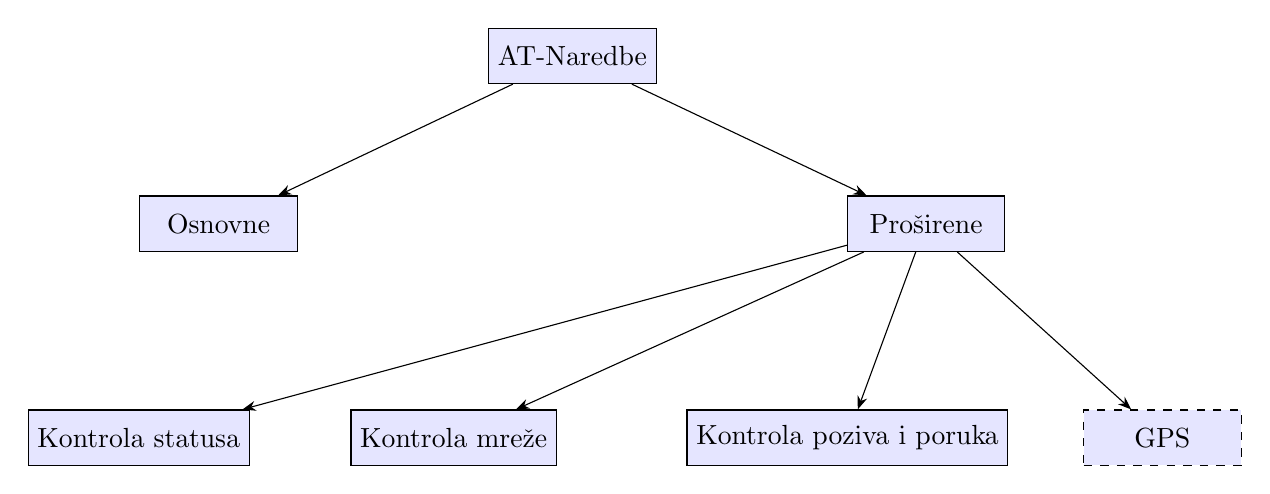
\begin{tikzpicture}[node distance=2cm, every node/.style={draw, fill=blue!10, rectangle, minimum height=2em, minimum width=2cm, text centered}, arrow/.style={-{Stealth}}]
    \node (at) {AT-Naredbe};
    \node (osnovne) [below left=of at, xshift=-1cm] {Osnovne};
    \node (prosirene) [below right=of at, xshift=1cm] {Proširene};
    \node (kontrolaStatusa) [below=of prosirene, xshift=-10cm] {Kontrola statusa};
    \node (kontrolaMreze) [below=of prosirene, xshift=-6cm] {Kontrola mreže};
    \node (kontrolaPoziva) [below=of prosirene, xshift=-1cm] {Kontrola poziva i poruka};
    \node (extraGPS) [below=of prosirene, xshift=3cm, draw=black, dashed] {GPS};

    \draw [arrow] (at) -- (osnovne);
    \draw [arrow] (at) -- (prosirene);
    \draw [arrow] (prosirene) -- (kontrolaStatusa);
    \draw [arrow] (prosirene) -- (kontrolaMreze);
    \draw [arrow] (prosirene) -- (kontrolaPoziva);
    \draw [arrow] (prosirene) -- (extraGPS);
  \end{tikzpicture}
  \caption{Klasifikacija AT-Naredbi}
  \label{fig:at-naredbe}
\end{figure}

\section{Prikupljanje lokacijskih informacija}
\label{dio:pokretljivost}

\begin{table}[h!]
  \centering
  \begin{tabular}{|c|c|}
      \hline
      \textbf{AT-Naredba} & \textbf{Opis naredbe} \\
      \hline
      AT+CGPS=1 & 3G/4G/5G prijenos i prijem signala \\
      \hline
      AT+CGPSINFO & 4G/5G prijenos i prijem signala \\
      \hline
      AT+CREG=2 & 3G/4G/5G prijem signala \\
      \hline
      AT+CREG? & 3G/4G/5G prijem signala \\
      \hline
  \caption{Popis AT-Naredbi korištenih za prikupljanje lokacijskih informacija}
  \label{tab:at_naredbe_lokacija}
\end{table}



%--- ZAKLJUČAK / CONCLUSION ----------------------------------------------------
\chapter{Zaključak}
\label{pog:zakljucak}

\blindtext


%--- LITERATURA / REFERENCES ---------------------------------------------------

% Literatura se automatski generira iz zadane .bib datoteke / References are automatically generated from the supplied .bib file
% Upiši ime BibTeX datoteke bez .bib nastavka / Enter the name of the BibTeX file without .bib extension
\bibliography{literatura}



%--- SAŽETAK / ABSTRACT --------------------------------------------------------

% Sažetak na hrvatskom
\begin{sazetak}
  Unesite sažetak na hrvatskom.

  \blindtext
\end{sazetak}

\begin{kljucnerijeci}
  prva ključna riječ; druga ključna riječ; treća ključna riječ
\end{kljucnerijeci}


% Abstract in English
\begin{abstract}
  Enter the abstract in English.
  
  \blindtext 
\end{abstract}

\begin{keywords}
  the first keyword; the second keyword; the third keyword
\end{keywords}


%--- PRIVITCI / APPENDIX -------------------------------------------------------

% Sva poglavlja koja slijede će biti označena slovom i riječi privitak / All following chapters will be denoted with an appendix and a letter
\backmatter

\chapter{The Code}

\Blindtext


\end{document}
